\chapter{Overview of the approach}
\label{chap:overview}

This case study concentrates on the connection between the design time, and the runtime domain. Our goal is to connect these two domains, and make a solution that generally can support the relation between the design, and runtime.

\begin{figure}[h]
	\centering
	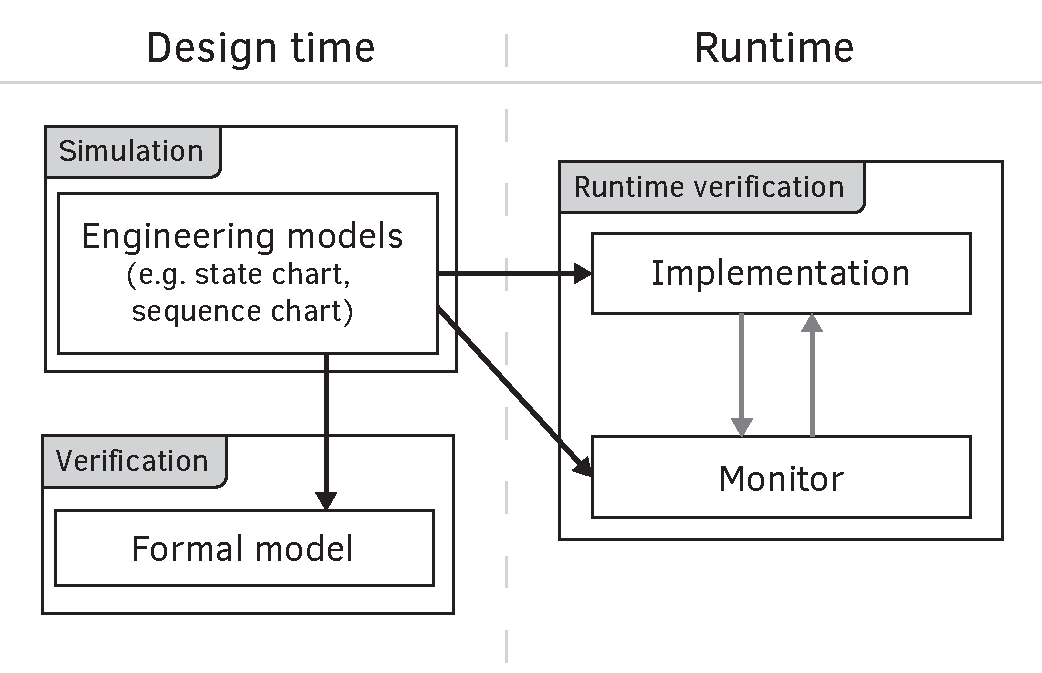
\includegraphics[width=0.75\linewidth]{include/figures/chapter_3/abstract_overview}
	\caption{Connection between runtime and design time elements}
	\label{fig:overview:abstract_overview}
\end{figure}

\cref{fig:overview:abstract_overview} depict the basic concept. We have three main transformation in the concept:
\begin{itemize}
	\item \textbf{Engineering model $\mapsto$ Formal model}: 
	\item \textbf{Engineering model $\mapsto$ Generated code}: From the verified model, we can generate an executable implementaion.
	\item \textbf{Engineering model $\mapsto$ Monitor}: Monitor the state of the implementation. If the execution reaches invalid states, the monitor detect it and forward the event of error detection into a higher level processor.
\end{itemize}
Solutions which connect two, or three elements of mapping are existing, but there are no tools which integrate all these in one tool with interchangeable formalisms. 
\\[1ex]

\noindent Let us consider the following example:

We want to design a system, where we have a model of our system, described by using a formalism (e.g. state chart, sequence chart), and we want to:
\begin{itemize}
	\item Generate the implementation from the model.
	\item Implement runtime verification into our implementation, by monitoring the application.
	\item We have multiple monitoring systems, and if a components verification state changes we want to react.
\end{itemize}

This example covers the usual needs of a distributed embedded safety logic. We need to formally verify the model, generate code, and monitor it. Our goal is to integrate all these solutions into a generic tool. With a centralized toolchain, a developer can make a system with less effort but with more robustness thanks to the verifiable, and automated steps.
\\[1ex]

\subsection{Hierarchical levels}

At the concept level